%---------------------------------------------------------------------------
%	Packages
%---------------------------------------------------------------------------
\documentclass[twocolumn]{article}
\usepackage[affil-it]{authblk}
\usepackage{amsmath}
\usepackage{background}
\usepackage{fancyhdr}
\usepackage[bottom]{footmisc}
\usepackage[left = 1cm ,right = 1cm, top = 2.5cm, bottom = 2.5cm]{geometry}
\usepackage{gensymb}
\usepackage{graphicx}
\usepackage[hidelinks]{hyperref}
\usepackage{indentfirst}
\usepackage{pgf}
\usepackage{pgfplots}
\usepackage{setspace}
\usepackage{tikz}
\usepackage{tkz-euclide}
\usepackage{url}
\usepackage{xcolor}
\usetikzlibrary{calc}
\usetikzlibrary{shapes.geometric, arrows}
\usetikzlibrary{decorations.pathreplacing}
\usetikzlibrary{decorations.pathmorphing}
\usetikzlibrary{decorations.markings}
\usepgfplotslibrary{units}
\pgfplotsset{compat=1.10}
\usetikzlibrary{arrows.meta}
\tikzset{>=Stealth}
\tikzset{snake it/.style={decorate, decoration=snake}}
%---------------------------------------------------------------------------
%	Header / Footer / Background
%---------------------------------------------------------------------------
\pagestyle{fancy}
\fancyhead[L]{Taylor Larrechea}
\fancyfoot[L]{PHYS 331}
\fancyhead[C]{X-Ray Diffraction of NaCl and KCl}
\fancyhead[R]{Colorado Mesa University}
\fancyfoot[R]{Final Report}
\backgroundsetup{
    scale = 1,
    angle = 0,
    opacity = 0.1,
    contents = {
    
\includegraphics[scale = 0.5, keepaspectratio]{Figures/CMU Seal.png}
    }
}
%---------------------------------------------------------------------------
%	Title And Author
%---------------------------------------------------------------------------
\title{\textbf{X-Ray Diffraction Of Table Salt}}
\author{Taylor Larrechea\footnote{Electronic Address: \texttt{tjlarrechea@mavs.coloradomesa.edu.}} \ and Edward McClain\footnote{Electronic Address: \texttt{epmcclain@mavs.coloradomesa.edu.}} \\
    Colorado Mesa University \\
    Department of Physical and Environmental Sciences \\
    1100 North Avenue \\
    Grand Junction, CO 81501-3122}
\date{April 15, 2019}
\begin{document}
\maketitle
%---------------------------------------------------------------------------
%	Abstract
%---------------------------------------------------------------------------
\begin{abstract}
Table salt and potassium chloride are examined via X-Ray Diffraction to determine the lattice spacing. The lattice spacing of the table salt and potassium chloride sample was calculated by measuring the angle of Diffraction from X-Rays. The experiment produced a lattice constant for table salt of $a=0.567(1)$ nm. The lattice constant for potassium chloride was found to be $a=0.524(3)$ nm. 
\end{abstract}
%---------------------------------------------------------------------------
%	Background
%---------------------------------------------------------------------------
\section*{Background}
X-Ray Diffraction is primarily used in identifying unknown crystalline structures such as minerals or inorganic compounds \cite{XRDDiffrac}. The identification of unknown solids is useful in geology, environmental science, and material science \cite{Qian}. The simplest structure is a simple cubic lattice, commonly found in materials such as table salt and potassium chloride. Figure 1 shows the simple cubic structure of table salt \cite{Ou}.
%---------------------------------------------------------------------------
%	Figure 1
%---------------------------------------------------------------------------
\begin{figure}[htbp]
\begin{center}
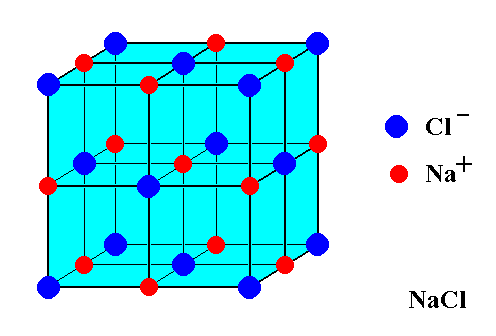
\includegraphics[width=0.35\textwidth]{Figures/PHYS 331 XRD Report Simple Cubic Rock Salt.png}
\caption{The simple cubic structure of table salt \cite{Ou}.}
\label{Fig1}
\end{center}
\end{figure}
\newpage
The side lengths in Figure 1 are all of the same length and orthogonal to one another hence the simple cubic name. Figure 2 shows the Diffraction of an X-Ray that is entering a crystalline structure such as table salt or sodium chloride.
%---------------------------------------------------------------------------
%	Figure 2
%---------------------------------------------------------------------------
\begin{figure}[htbp]
\begin{center}
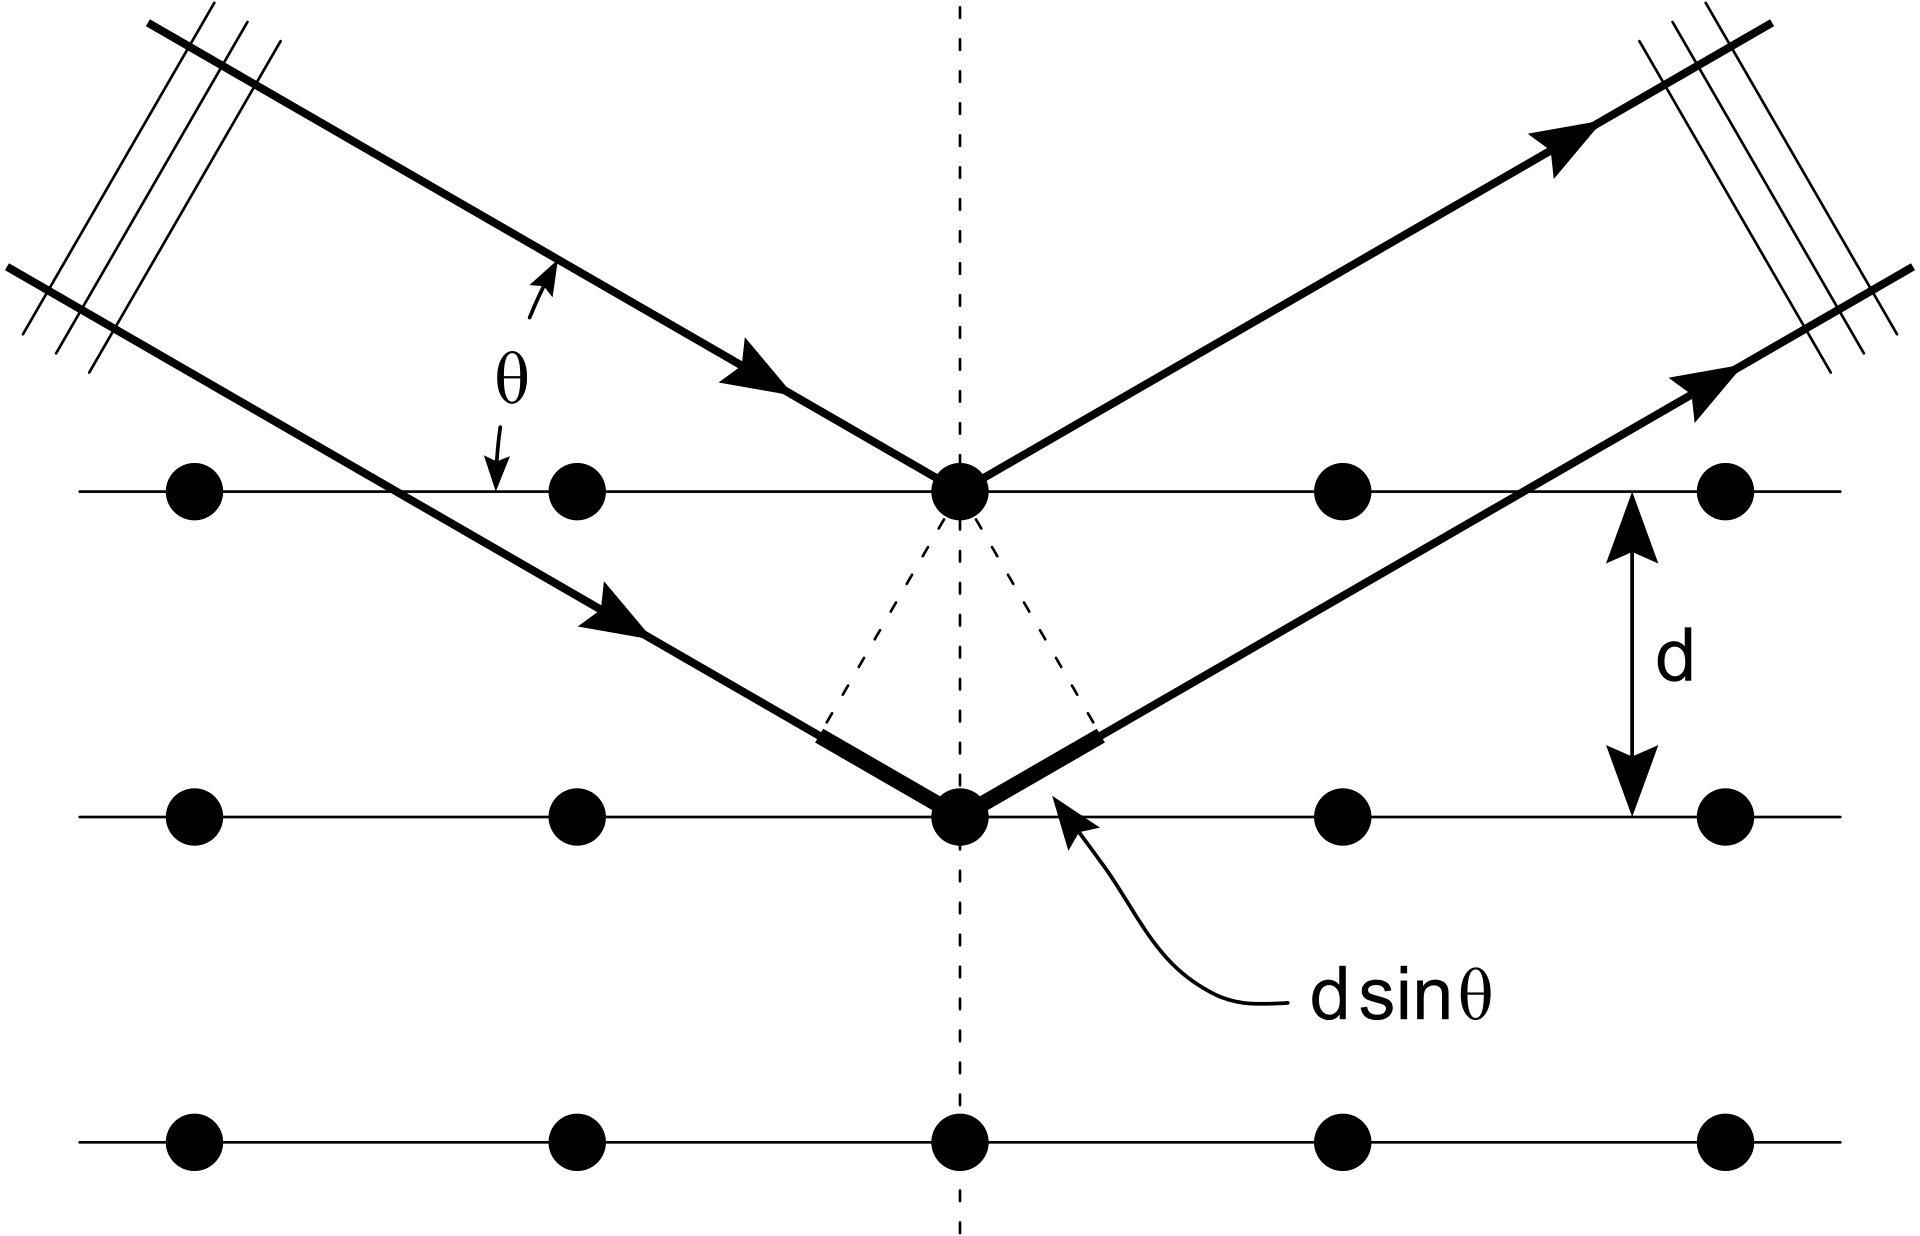
\includegraphics[width=0.35\textwidth]{Figures/PHYS 331 XRD Report XRD.png}
\caption{The X-Ray Diffraction inside a crystalline structure \cite{X-RayCryst}. The distance between atom planes is \textit{d}.}
\label{Fig2}
\end{center}
\end{figure}
Figure 2 shows the X-Ray Diffraction distance once they enter a crystalline structure. This distance is contingent upon the angle of diffraction ($\theta$ as seen in Figure 2 above), the wavelength of the light $\lambda$, and the order of magnitude of the wavelength of light $n$. This distance occurs in Bragg's law and is formally
%---------------------------------------------------------------------------
%	Equation 1
%---------------------------------------------------------------------------
\begin{equation}\label{1}
2d\sin{\theta}=n\lambda
\end{equation}
where $d$ is the distance between lattice planes. In order to calculate the lattice constant of table salt and potassium chloride in this experiment we need to know the Miller indices\footnote{Miller indices are usually represented in a form of (\textit{h},\textit{k},\textit{l}). The \textit{h}, \textit{k}, and \textit{l} can vary in different letters and symbols depending on the author of the report or article.} for both. The Miller indices of a substance are the inverse of the intercepts of the of the plane of a substance with the a unit cell \cite{WikiCrystal}. A visual representation of Miller indices can be seen in Figure 3.
%---------------------------------------------------------------------------
%	Figure 3
%---------------------------------------------------------------------------
\begin{figure}[htbp]
\begin{center}
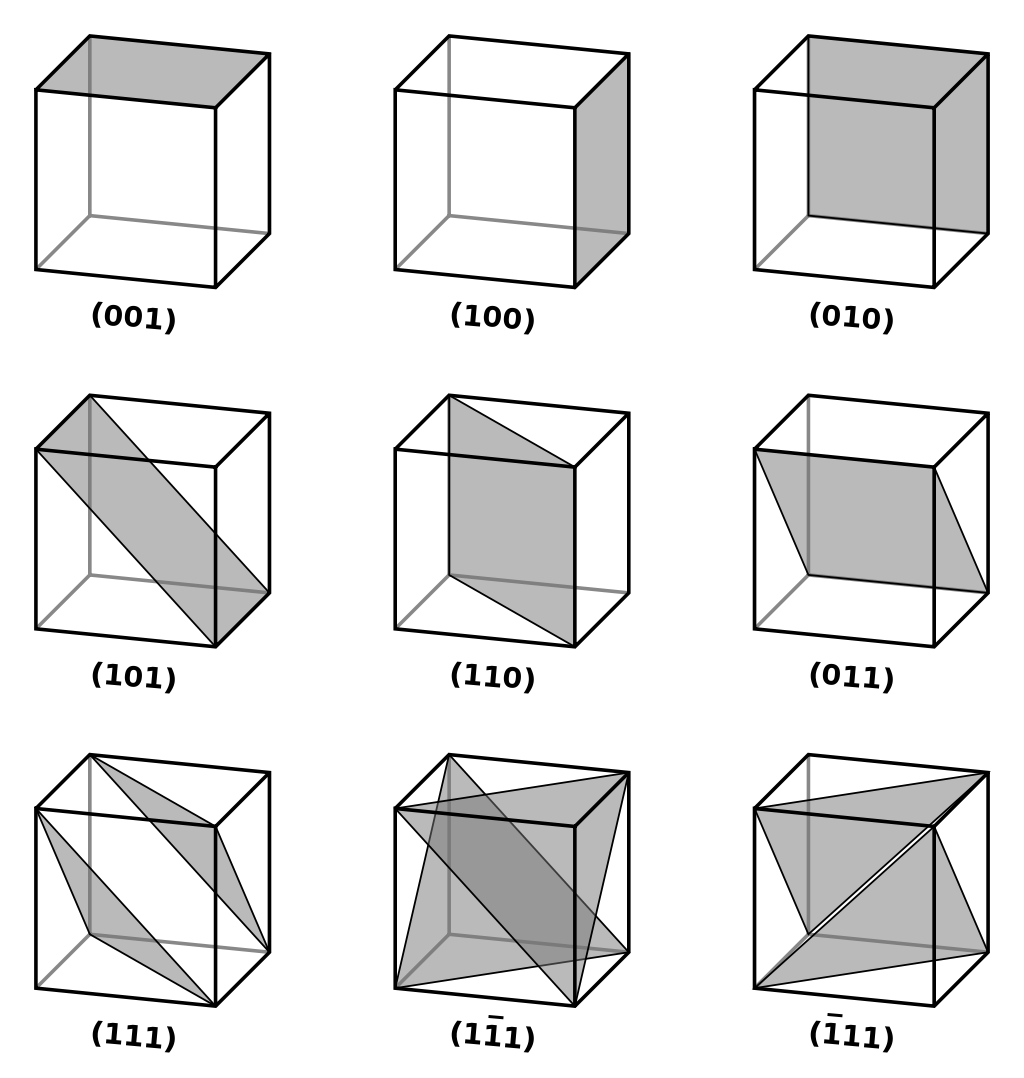
\includegraphics[width=0.35\textwidth]{Figures/PHYS 331 XRD Report Miller Indices.png}
\caption{Physical representation of the numbers seen in a Miller index \cite{WikiCrystal}.}
\label{Fig3}
\end{center}
\end{figure}
\newpage
The Miller indices come from which plane of the simple cubic is being intercepted. After knowing the Miller indices of table salt and potassium chlordie we can proceed to calculating the lattice constant. In compliance with equation (1), the lattice constant is calculated via
%---------------------------------------------------------------------------
%	Equation 2
%---------------------------------------------------------------------------
\begin{equation}\label{2}
a=d\sqrt{h^2+k^2+l^2}
\end{equation}
where \textit{h}, \textit{k}, and \textit{l} are contingent upon the geometry of the substance that is being observed \cite{X-RayCryst}. The $d$ distance in equation (1) could be calculated once $n$ was set equal to one since the $\theta$ value could be measured with the instrumentation.
%---------------------------------------------------------------------------
%	Experimental
%---------------------------------------------------------------------------
\section*{Experimental}
X-Ray Diffraction patterns were acquired using a Rigaku Miniflex diffractometer equipped with a copper k-$\alpha$ source with a wavelength of $\lambda=0.1544256$ nm and a glass slide to hold the Kroger brand non-iodized table salt or potassium chloride sample. The first step was to place the sample on the glass slide with ethanol sprayed on top and then placed inside the Rigaku Miniflex. After the slide was inserted and other settings were selected the Rigaku Miniflex started generating X-Rays that were to be incident on the table salt and potassium chloride sample. The detector inside the Rigaku Minflex measured the deflection angle of these X-Rays in a form of 2$\theta$. 
%---------------------------------------------------------------------------
%	Data And Results
%---------------------------------------------------------------------------
\section*{Data and Results}
The Diffraction pattern of the table salt sample with the corresponding Miller indices for each Diffraction peak can be seen in Figure 4 \cite{Lecture}.
%---------------------------------------------------------------------------
%	Figure 4
%---------------------------------------------------------------------------
\begin{figure}[htbp]
\begin{center}
\begin{tikzpicture}[scale=1.0]
    \begin{axis}[
        ylabel=Intensity,
        xlabel=2$\theta$,
        x unit=degrees, y unit=A.U.,
        xmin=20, xmax=80,
        %ymin=0, ymax=80,
        ytick=\empty,
        yticklabels={,,},]
    \addplot[mark=none] table [x=theta, y=intensity, col sep=comma]{PHYS 331 XRD Data (NaCl).txt};
    \node at (axis cs:27.35,700) {\small (111)};
    \node at (axis cs:36,2500) {\small (200)};
    \node at (axis cs:45.5,1500) {\small (220)};
    \node at (axis cs:51.8,350) {\small (311)};
    \node at (axis cs:56.4,1200) {\small (222)};
    \node at (axis cs:66.0,800) {\small (400)};
    \node at (axis cs:75.1,1500) {\small (420)};
    \end{axis}
\end{tikzpicture}
\label{Fig4}
\caption{X-Ray Diffraction of table salt with the corresponding Miller indices for each diffraction peak.}
\end{center}
\end{figure}
\newline
Figure 4 shows the intensity versus the $2\theta$ angle of diffraction for the table salt sample. There are seven distinct peaks from left to right that are created during this phenomena which will be used to calculate the diffraction distance and eventually the lattice constant. These peaks then had their angles of which they occurred at extracted and used to find a distance for the lattice spacing between respective atom planes of the table salt sample. Once $d$ in equation (1) was known it could be used with the correct Miller index of the respective peak to determine the lattice constant of table salt. Table 1 shows the data found in Figure 4. The abbreviation, ``M.I." is short for Miller index in the following tables.
%---------------------------------------------------------------------------
%	Table 1
%---------------------------------------------------------------------------
\begin{table}[htp]
\begin{center}
\begin{tabular}{|c|c|c|}
	\hline \small{\textbf{Peak \& M.I.}} & \small{\textbf{Angle $2\theta$ ($^{\circ}$)}} & \small{\textbf{Intensity (A.U.)}} \\ \hline
    (111)& $27.35\pm0.00$ & $126.7\pm4.850$ \\ \hline
    (200)& $31.39\pm0.00$ & $303.7\pm13.74$ \\ \hline
    (220)& $45.39\pm0.00$ & $654.9\pm9.580$ \\ \hline
    (311)& $53.80\pm0.00$ & $37.20\pm3.260$ \\ \hline
    (222)& $56.39\pm0.00$ & $471.4\pm8.170$ \\ \hline
    (400)& $65.98\pm0.00$ & $284.1\pm6.610$ \\ \hline
    (420)& $75.15\pm0.00$ & $475.9\pm8.390$ \\ \hline 
\end{tabular}
\caption{Data for X-Ray Diffraction of table salt. The Miller Indices were unknown for peaks 5-7.}
\end{center}
\label{default}
\end{table}%
\newline
The data seen in Table 1 above was analyzed with a peak fitting software called Fityk using Gaussian peaks \cite{Fityk}. Using equation (2), the lattice constant of table salt can be calculated with the data found in Table 1. The lattice constant calculations can be seen in Table 2.
%---------------------------------------------------------------------------
%	Table 2
%---------------------------------------------------------------------------
\begin{table}[htp]
\begin{center}
\begin{tabular}{|c|c|c|}
	\hline \small{\textbf{Peak \& M.I.}} &\small{\textbf{$d$ (nm)}} & \small{\textbf{$a$ (nm)}} \\ \hline
	(111) & 0.326 & 0.565 \\ \hline
	(200) & 0.285 & 0.570 \\ \hline
	(220) & 0.200 & 0.566 \\ \hline
	(311) & 0.171 & 0.567 \\ \hline
	(222) & 0.163 & 0.566 \\ \hline
	(400) & 0.142 & 0.567 \\ \hline
	(420) & 0.127 & 0.566 \\ \hline
\end{tabular}
\caption{Lattice constant calculations from each peak for table salt.}
\end{center}
\label{default}
\end{table}%
\newline
Taking an average and finding the standard deviation of the lattice constants found in Table 2, the final calculated lattice constant for table salt from this experiment is
%---------------------------------------------------------------------------
%	Equation 3
%---------------------------------------------------------------------------
\begin{equation}
a_{NaCl}=0.567(1) \ nm.
\end{equation}
The formal value for the lattice constant of sodium chloride is $a=0.564$ nm \cite{WikiLattice}. This reveals that our value is slightly out of range due to a calibration error in the equipment that was being used. The same procedure was ran for potassium chloride that was used for table salt. The X-Ray Diffraction pattern of potassium chloride and the correct corresponding Miller indices of each peak can be seen in Figure 5 \cite{Lin}.
%---------------------------------------------------------------------------
%	Figure 5
%---------------------------------------------------------------------------
\begin{figure}[htbp]
\begin{center}
\begin{tikzpicture}[scale=1.0]
    \begin{axis}[
        ylabel=Intensity,
        xlabel=2$\theta$,
        x unit=degrees, y unit=A.U.,
        xmin=20, xmax=80,
        %ymin=0, ymax=80,
        ytick=\empty,
        yticklabels={,,},]
    \addplot[mark=none] table [x=theta, y=intensity, col sep=comma]{PHYS 331 XRD Data (KCl).txt};
    \node at (axis cs:33.0,4400) {\small (200)};
    \node at (axis cs:41.07,2500) {\small (220)};
    \node at (axis cs:50.70,800) {\small (222)};
    \node at (axis cs:59.2,1100) {\small (400)};
    \node at (axis cs:66.9,1700) {\small (420)};
    \node at (axis cs:74.2,1100) {\small (422)};
    \end{axis}
\end{tikzpicture}
\label{Fig4}
\caption{X-Ray Diffraction of potassium chloride with the corresponding Miller indices for each diffraction peak.}
\end{center}
\end{figure}
\newline
There are six distinct peaks that arise from the X-Ray Diffraction of potassium chloride. Using the data and the Miller indices in Figure 5, Table 3 is constructed to relay the X-Ray Diffraction for potassium chloride.
%---------------------------------------------------------------------------
%	Table 3
%---------------------------------------------------------------------------
\begin{table}[htp]
\begin{center}
\begin{tabular}{|c|c|c|}
	\hline \small{\textbf{Peak \& M.I.}} & \small{\textbf{Angle ($^{\circ}$)}} & \small{\textbf{Intensity (A.U.)}} \\ \hline
	(200)& $28.89\pm0.00$ & $1848.0\pm50.550$ \\ \hline
	(220)& $41.07\pm0.00$ & $730.8\pm32.23$ \\ \hline
	(222)& $50.70\pm0.01$ & $151.2\pm15.98$ \\ \hline
	(400)& $59.21\pm0.01$ & $356.5\pm23.45$ \\ \hline
	(420)& $66.94\pm0.01$ & $572.8\pm28.94$ \\ \hline
	(422)& $74.25\pm0.01$ & $275.1\pm20.96$ \\ \hline
\end{tabular}
\caption{Data for X-Ray Diffraction of potassium chloride.}
\end{center}
\label{default}
\end{table}%
\newline
Using the same procedure that was used for table salt the lattice spacing of potassium chloride can be seen in Table 4.
%---------------------------------------------------------------------------
%	Table 4
%---------------------------------------------------------------------------
\begin{table}[htp]
\begin{center}
\begin{tabular}{|c|c|c|}
	\hline \small\textbf{{Peak}} &\small{\textbf{$d$ (nm)}} & \small{\textbf{$a$ (nm)}} \\ \hline
	1 & 0.309 & 0.618 \\ \hline
	2 & 0.220 & 0.622 \\ \hline
	3 & 0.180 & 0.624 \\ \hline
	4 & 0.156 & 0.624 \\ \hline
	5 & 0.140 & 0.626 \\ \hline
	6 & 0.128 & 0.627 \\ \hline
\end{tabular}
\caption{Lattice constant calculations from each peak for potassium chloride.}
\end{center}
\label{default}
\end{table}%
\newline
Taking the averages of the lattice constants found in Table 4, our final value for the lattice constant of potassium chloride is
%---------------------------------------------------------------------------
%	Equation 4
%---------------------------------------------------------------------------
\begin{equation}
a_{KCl}=0.624(3) \ nm.
\end{equation}
The formal value for the lattice constant of potassium chloride is $a=0.629$ nm \cite{WikiLattice}. This once again shows that our equipment is in need of calibrating.
%---------------------------------------------------------------------------
%	Conclusion
%---------------------------------------------------------------------------
\section*{Conclusion}
In this experiment X-Ray Diffraction was used to find the lattice constant of table salt and potassium chloride. The lattice constant for table salt was calculated to be $a_{NaCl}=0.567(1)$ nm where the formal value is $a=0.564$ nm \cite{WikiLattice}. This discrepancy is largely in part due to equipment needing to be calibrated. The same procedure was conducted on potassium chloride and the lattice constant was found to be $a_{KCl}=0.624(3)$ nm where the formal value is  $a=0.629$ nm \cite{WikiLattice}. The lattice constant for potassium chloride is also outside the range of the formal value once again caused due to a lack of calibration in the equipment. More accurate calculations of the lattice constants could be achieved with better calibrated equipment. For further investigations of X-Ray Diffraction see references [1]-[13].
%---------------------------------------------------------------------------
%	Bibliography
%---------------------------------------------------------------------------
\newpage
\begin{thebibliography}{13}
\bibitem{WikiBraggs}
Bragg's law. (2018, December 03). Retrieved April 6, 2019, from \url{https://en.wikipedia.org/wiki/Bragg's_law}.
\bibitem{WikiCrystal}
Crystal Structure. Wikipedia, Wikimedia Foundation, 18 Feb. 2019, \url{en.wikipedia.org/wiki/Crystal_structure}.
\bibitem{WikiGauss}
Gaussian Function. Wikipedia, Wikimedia Foundation, 15 Mar. 2019, \url{en.wikipedia.org/wiki/Gaussian_function}.
\bibitem{Ionic}
Ionic Solids. (n.d.). Retrieved from \url{http://nersp.nerdc.ufl.edu/~wsawyer/atoms/chapter4/chapter4.html}.
\bibitem{WikiLattice}
Lattice Constant. Wikipedia, Wikimedia Foundation, 11 Mar. 2019, \url{en.wikipedia.org/wiki/Lattice_constant}.
\bibitem{Lecture}
Lecture presented at Physical Methods For Characterizing Solids. (2019, April 6).
\bibitem{Lin}
Lin, Kuen-Song \& Mai, Yao-Jen \& Li, Shin-Rung \& Shu, Chia-Wei \& Wang, Chieh-Hung. (2012). Characterization and Hydrogen Storage of Surface-Modified Multiwalled Carbon Nanotubes for Fuel Cell Application. Journal of Nanomaterials. 2012. 10.1155/2012/939683. 
\bibitem{Moroz}
Moroz, E. M. (2017). Possibilities of powder X-ray Diffraction methods in determining structural characteristics of carbon materials. Journal of Structural Chemistry, 58(8), 1510–1514. \url{https://doi.org/10.1134/S0022476617080054}.
\bibitem{Ou}
Oushida oushida 209145, Curt F.Curt F. 15.7k13688, JerkxesJerkxes 493, Karsten TheisKarsten Theis 4, \& Andseliskandselisk 19.1k661125. (2015, July 1). Number of atoms in NaCl unit cell. Retrieved April 11, 2019, from \url{https://chemistry.stackexchange.com/questions/34119/number-of-atoms-in-nacl-unit-cell}.
\bibitem{Fityk}
Wojdyr, Marcin. Fityk: a General-Purpose Peak Fitting Program. Journal of Applied Crystallography, 10 Sept. 2010, \url{onlinelibrary.wiley.com/iucr/doi/10.1107/S0021889810030499}.
\bibitem{Qian}
Qian Zhang, Fei Qin, Jing Jing Niu, \& Xiang Wu. (2018). High-pressure investigation on prehnite: X-ray Diffraction and Raman spectroscopy. High Temperatures -- High Pressures, 47(3), 213–221. Retrieved from \url{http://search.ebscohost.com/login.aspx?direct=true&db=a9h&AN=131005884&site=eds-live&scope=site}.
\bibitem{X-RayCryst}
X-Ray Crystallography. Wikipedia, Wikimedia Foundation, 9 Mar. 2019, \url{en.wikipedia.org/wiki/X-ray_crystallography}.
\bibitem{XRDDiffrac}
X-Ray Powder Diffraction (XRD). Techniques, 19 Mar. 2019, \url{serc.carleton.edu/research_educationgeochemsheets/techniques/XRD.html}.
\end{thebibliography}
\end{document}